\documentclass{article}
\usepackage{hyperref}
\usepackage{fancyhdr}
\usepackage{graphicx}
\usepackage{amsmath}
\usepackage{amssymb}
\usepackage{float}
\usepackage{enumitem}
\usepackage{mathtools}

% if you want to create a new list from scratch
\newlist{alphalist}{enumerate}{1}
% in that case, at least label must be specified using \setlist
\setlist[alphalist,1]{label=\textbf{\alph*.}}

% \graphicspath{{images/}}
\pagestyle{fancy}
\title{EE 271: Final Project Inference Engine on FPGA}
\author{Jay Pankaj Patel}
\date{\today}

\begin{document}
\maketitle
\tableofcontents
\newpage

\section{Building Blocks}
For our inference implementation, I am considering using Convolutional Neural Networks (CNNs). They are an algorithm used to recognize patterns in data. I believe the target data should be handwritten digits from 0--9. Neural networks are built using a collection of neurons organized into layers, each with their own weights and biases. The building blocks of CNNs are the following:
\begin{itemize}
  \item \textbf{Tensor} -- can be thought of as an $n$-dimensional matrix. We need to decide how big to make our tensor. I was considering making it smaller, like three dimensions, because our goal is to perform simple classification.
  \item \textbf{Neuron} -- is a mathematical function that takes multiple inputs and gives a single output.
  \item \textbf{Layer} -- is simply defined as a collection of neurons.
  \item \textbf{Kernel Weights and Biases} -- unique to each neuron and are determined during the training phase of our network. We will train the model on a computer and extract the weights and biases to the FPGA for inference.
  \item \textbf{Differentiable Score Function} -- represented as class scores on the output layer.
\end{itemize}
These are the high-level components needed. Using this knowledge, let’s go over the proposed design.

\section{Design}
Our neural network is going to be as simple as possible because the emphasis of this project will be optimizing the operations required for the model to run. Hence, we are using the "Hello World" equivalent of Machine Learning. Our architecture is as follows. 

\subsection{Architecture}
Our design will take a \textbf{28×28 grayscale image} as input.

After:
\begin{itemize}
  \item A \textbf{convolution layer} will be used to apply 8 kernels to the input, generating \textbf{8 feature maps of size 26×26}, which are then passed to a max-pooling layer.
  \item A \textbf{max-pooling layer} will reduce the \textbf{spatial dimensions} of each feature map from \textbf{26×26 to 13×13}, maintaining 8 feature maps, and will pass the results to the softmax layer.
  \item For training, a \textbf{softmax layer} will process the \textbf{flattened feature maps} and produce \textbf{10 probability values}, each representing the likelihood of the image belonging to one of the 10 classes (digits 0–9).
  \item For the inference and implementation on hardware, a \textbf{hardmax layer} will be used as implementing softmax on hardware is resource intensive and will increase development time.
\end{itemize}

Here is a visual representation of these processes.
\begin{figure}[H]
  \begin{center}
    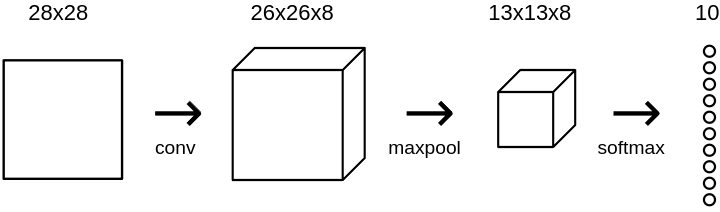
\includegraphics[width=0.95\textwidth]{figures/arch_vis_training}
  \end{center}
  \caption{Visual representation of the CNN layers that will implemented as training in software}\label{fig:cnn_arch}
\end{figure}
\begin{figure}[H]
  \begin{center}
    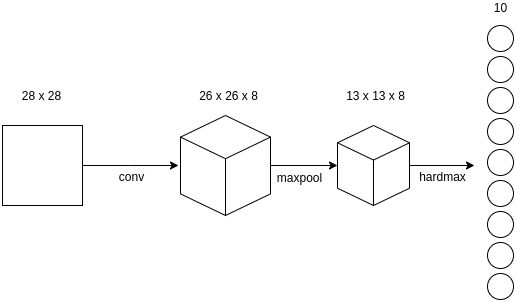
\includegraphics[width=0.95\textwidth]{figures/arch_vis}
  \end{center}
  \caption{Visual representation of the CNN layers that will implemented in hardware}\label{fig:cnn_arch}
\end{figure}
\newpage 
\subsection{Model}
A Python golden model has been created and should be used to validate the FPGA implementation. The Python model is not optimized for hardware, and operations should be adjusted for efficient computation on the FPGA. The model has been pre-trained in Python, and the trained weights and biases will be ported to the FPGA for inference. FPGA-specific design considerations will be discussed after detailing the theory behind each layer.

\subsection{Convolutional Layer Design}
\subsubsection{Background}
\begin{itemize}
  \item \textbf{What is a feature?} \\
    A feature is an individual measurable property that a model uses to make a prediction or classification.
  \item \textbf{What is a feature map?} \\
    A feature map is the output produced when a convolutional kernel extracts relevant features from an input. In this field, the 'filter' is referred to as a \emph{kernel}. Hence, I will be using "kernel" from this point forward.
  \item \textbf{What is convolution?} \\
    Convolution, in a mathematical sense, is an operation performed on two functions that produces a third function. The mathematical operation is defined as the integral of the two functions after one of them is reflected about the y-axis and shifted. Mathematically:
\end{itemize}

\subsection{Equations}
\begin{align*}
  \left( f  * g \right) \left( t \right) &= \int_{-\infty}^{\infty} f \left( \tau \right) g \left( t - \tau \right) \, d\tau
\end{align*}

Graphically:
\begin{figure}[H]
  \begin{center}
    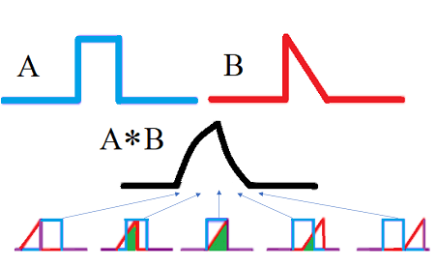
\includegraphics[width=0.5\textwidth]{figures/math_con}
  \end{center}
  \caption{Convolution of two functions A (red) and B (blue) producing a third function describing the overlap (green)}\label{fig:convolution}
\end{figure}

Since we are dealing with discrete systems, convolution is defined using summation instead of an integral:

\begin{align*}
  \left( f * g \right) \left[ n \right] &= \sum_{m = -\infty}^{\infty} f \left[ m\right] g \left[ n-m \right]
\end{align*}

In CNNs, the most computationally expensive operation is the convolution layer. The convolution of the input feature map with the kernel results in an output feature map:

\begin{align*}
  \Aboxed{  y'_j = f \left( \sum_{i \in M_j}^{} x^{l-1}_{i}  * k^l_{ij} + b^l_{j}\right)}
\end{align*}

Where:
\begin{itemize}
  \item \( y^{l}_j \) : Feature map of the \( j \)th convolution kernel result of the \( l  \)th layer.
  \item \( M_{j} \) : Represents the selection of the previous input feature map by the current convolution.
  \item \( x_{i }^{l-1} \): Represents the previous input feature map.
  \item \( k_{ij}^l  \): Represents the \( i  \)th weighting coefficient of the \( j  \)th convolution of the \( l  \)th layer.
  \item \( b^{l }_j \) : Represents the bias parameter of the \( j  \)th convolution kernel of the \( l  \)th layer.
  \item \( f \) : The nonlinear activation function.
\end{itemize}

\subsection{Pooling Layer Design}
\subsubsection{Background}
\begin{itemize}
  \item \textbf{What is pooling?} \\
    Pooling is a technique used to downsample feature maps by aggregating adjacent values.
  \item \textbf{Why pooling?} \\
    Neighboring pixels in images tend to have similar values, leading to redundant information. Pooling reduces this redundancy while retaining important features.
  \item \textbf{How is pooling done?} \\
    Pooling is implemented using a max, min, or average value comparison over a small region.
\end{itemize}

\subsection{Pooling Equation}
A 3×3 convolution computes each output pixel using a weighted sum of a 3×3 region from the input:

\begin{align*}
  \Aboxed{ Y(i, j) &= \sum_{m=0}^{2} \sum_{n=0}^{2} X(i+m, j+n) \cdot W(m, n)}
\end{align*}

Where:
\begin{itemize}
  \item \( X(i, j) \) is the input feature map (28×28).
  \item \( W(m, n) \) is the 3×3 convolution kernel (filter).
  \item \( Y(i, j) \) is the output feature map after convolution.
\end{itemize}

Valid padding means no padding is added, so the output size is:

\[
(28-3+1) \times (28-3+1) = 26 \times 26
\]
And we repeat this 8 times because we have 8 kernels. Hence our final output will be 26 x 26 x 8.

\subsection{Softmax Layer Design}
\subsubsection{Background} 
\begin{itemize}
  \item \textbf{What is an activation function?}
    An activation function allows our model to achieve non-linearity as most things in real life are not a linear equation. By doing so, it allows our model to achieve higher accuracies.
  \item \textbf{What is softmax?} 
    Softmax is an activation function that converts an arbitrary set of numbers into a probability distribution. 
  \item \textbf{Why Softmax?} 
      Softmax is useful when you have a multi-class model as we do here, (0-9 are different classes). 
\end{itemize}

\subsection{Softmax Equation} 
Mathematically, given an input vector \( x = [x_1, x_2, ..., x_n] \), the Softmax function is defined as:

\begin{align*}
  \Aboxed{s(x_i) = \frac{e^{x_i}}{\sum_{j=1}^{n} e^{x_j}}}
\end{align*}
where:
\begin{itemize}
    \item \( x_i \) represents the raw input (logit) for class \( i \).
    \item \( e^{x_i} \) represents exponentiation of the input values.
    \item The denominator is the \textbf{sum of exponentials} over all input values.
    \item The function ensures that all outputs sum to 1.
\end{itemize}
\subsubsection{Sample Calculation} 
\begin{enumerate}
    \item Compute exponentials:
    \[
    e^{-1} = 0.368, \quad e^0 = 1, \quad e^3 = 20.09 \\
    \quad e^5 = 148.41
    \]

    \item Compute denominator (sum of exponentials):
    \[
    0.368 + 1 + 20.09 + 148.41 = 169.87
    \]

    \item Compute Softmax probabilities:
    \begin{align*}
      s(-1) &= \frac{0.368}{169.87} = 0.002\\ 
      s(0) &= \frac{1}{169.87} = 0.006\\ 
      s(3) &= \frac{20.09}{169.87} = 0.118\\ 
      s(5) &= \frac{148.41}{169.87} = 0.874
    \end{align*}
\end{enumerate}

Thus, the final probability distribution is:
\[
[0.002, 0.006, 0.118, 0.874]
\]

This means the model is \textbf{87.4\% confident in class 5} and assigns lower probabilities to other classes.

\subsection{Hardmax Layer Design}
\subsubsection{Background} 
\begin{itemize}
  \item \textbf{What is hardmax?}  
    Hardmax is a function that converts a set of values into a one-hot encoded vector, where only the index with the highest value is set to 1 and all others are set to 0.
  \item \textbf{Why Hardmax?}  
    Hardmax is useful during inference when we want to make a final decision and select the most likely class. It is deterministic and discrete, which makes it appropriate for classification output.
\end{itemize}

\subsection{Hardmax Equation}
Given an input vector \( x = [x_1, x_2, ..., x_n] \), the Hardmax function outputs a vector \( h = [h_1, h_2, ..., h_n] \), where:

\[
h_i =
\begin{cases}
1 & \text{if } i = \arg\max_j x_j \\
0 & \text{otherwise}
\end{cases}
\]

\noindent where:
\begin{itemize}
    \item \( x_i \) represents the raw input (logit) for class \( i \).
    \item \( \arg\max_j x_j \) returns the index of the maximum value in the input vector.
    \item The result is a one-hot vector with a 1 at the index of the largest value.
\end{itemize}

\subsubsection{Sample Calculation} 
\begin{enumerate}
    \item Input vector:
    \[
    x = [-1,\ 0,\ 3,\ 5]
    \]

    \item Find index of maximum value:
    \[
    \arg\max(x) = 3 \quad \text{(since } x_4 = 5 \text{ is largest)}
    \]

    \item Convert to one-hot encoding:
    \[
    h = [0,\ 0,\ 0,\ 1]
    \]
\end{enumerate}

\noindent Thus, the final hardmax output is:
\[
[0,\ 0,\ 0,\ 1]
\]

\noindent This means the model predicts class 3 with full confidence and disregards the other classes completely.

\section{Hardware Design}
\subsection{Number Representation}
\subsubsection{Qm.n format} 
Q format is a standardized way to represent fractional numbers in hardware. We cannot use floating point as the FPGA we are targeting does not have enough resources to implement a floating point model. In Qm.n format, \emph{m} is the number of bits that will be used to represent the whole number portion of the number. \emph{n} is the number of bits that will be used to represent the fractional portion of the number. Based on the hardware used, it was determined that 16 bits was enough to fit our design on a FPGA.
\subsection{Fixed-Point Format Selection}
After running the software model, it was determined that the number range that is present in our system is between \textbf{-3.1 to 3.1}. To represent this in hardware we need to use
To represent numbers in the range \(-3.1\) to \(+3.1\) using fixed-point arithmetic with a 16-bit word, we select an appropriate Q-format that maximizes precision while avoiding overflow.

\subsubsection*{Bit Allocation}

The 16-bit word must include:
\begin{itemize}
  \item 1 sign bit (for two's complement representation)
  \item \(m\) integer bits
  \item \(n\) fractional bits
\end{itemize}

Thus, we must satisfy:
\[
1~(\text{sign}) + m~(\text{integer}) + n~(\text{fraction}) = 16
\]

\subsubsection*{Determining Integer Bits}

To safely represent the maximum magnitude value \(3.1\), we need:
\[
2^m > 3.1
\]
Solving this, we find:
\[
m = 2 \quad \text{since} \quad 2^2 = 4 > 3.1
\]

\subsubsection*{Fractional Bits}

Given \(m = 2\) and 1 sign bit, the remaining bits for the fractional part are:
\[
n = 16 - 1 - 2 = 13
\]

\subsubsection*{Selected Q Format}

We choose the Q-format:
\[
\textbf{Q2.13}
\]

This format uses:
\begin{itemize}
  \item 1 sign bit
  \item 2 integer bits
  \item 13 fractional bits
\end{itemize}

\subsubsection*{Representable Range and Precision}

The Q2.13 format can represent values in the approximate range:
\[
[-2^2, 2^2 - 2^{-13}] = [-4, 3.99987793]
\]

The smallest positive value (resolution) is:
\[
2^{-13} \approx 0.00012207
\]

This ensures that values within \([-3.1, +3.1]\) can be accurately represented without overflow, with high fractional precision.
\subsection{Multiply Accumulate (MAC) Unit}

In Convolutional Neural Networks (CNNs), the majority of computations come from convolution and fully connected layers. These layers apply a large number of dot products between learned filters (weights) and input data. Each dot product is computed through a series of \textbf{multiply-accumulate (MAC)} operations, which follow the form:

\[
\text{MAC: } a \times b + c
\]

where $a$ is a weight, $b$ is an input value, and $c$ is the accumulation result (running sum).

\subsubsection*{Fixed-Point Constraints in MAC Design}

When using fixed-point numbers—such as the Q2.13 format, where 16-bit signed integers represent values in the range $[-4.0, 3.9998]$—the MAC unit must handle several constraints:

\subsubsection{Saturation Handling} 
Without saturation, any arithmetic overflow may wrap around due to two's complement behavior. For instance, a small positive overflow can produce a large negative result, leading to incorrect predictions. Saturation logic ensures that results exceeding the representable range are clamped to the maximum or minimum:

\begin{verbatim}
if (result > MAX_Q213)
    output = MAX_Q213;
else if (result < MIN_Q213)
    output = MIN_Q213;
else
    output = result;
\end{verbatim}

\paragraph{Truncation and Rescaling} Multiplying two Q2.13 values produces a Q4.26 intermediate result:

\[
Q2.13 \times Q2.13 = Q4.26
\]

To convert this back to Q2.13, the result must be truncated by shifting 13 bits to the right:

\begin{verbatim}
wire signed [31:0] full_product = a * b;
wire signed [15:0] scaled_product = full_product >>> 13;
\end{verbatim}

This truncation maintains numerical scale and fits the result into 16 bits.

\subsubsection*{Example 1: Convolution Filter on MNIST Input}

For an 8-filter $3 \times 3$ convolution on a $28 \times 28$ grayscale MNIST image, each output pixel requires:

\[
\sum_{i=1}^{9} w_i \cdot x_i
\]

This results in $9 \times 26 \times 26 \times 8 = 48,672$ MAC operations per image in the first layer. Fixed-point MAC units allow this to be computed efficiently using parallelism and pipelining.

\subsubsection*{Example 2: Fully Connected Output Layer}

In a final dense layer mapping to 10 output classes, with 1352 inputs (e.g., $13 \times 13 \times 8$), the number of MACs is:

\[
1352 \times 10 = 13,520
\]

All these operations must respect Q2.13 truncation and saturation constraints to ensure valid inference results.

\subsubsection*{Summary}

CNN inference relies heavily on MAC operations. Fixed-point formats like Q2.13 are ideal for resource-constrained hardware platforms. Proper MAC unit design must include:

\begin{itemize}
    \item \textbf{Saturation logic} to prevent overflow wraparound
    \item \textbf{Truncation logic} to maintain fixed-point scale
\end{itemize}

\subsection{Bus Design}
\subsubsection{Component Interface: AXI-Stream}
\textbf{AXI-Stream} is a lightweight and high-throughput unidirectional data transfer protocol derived from the Advanced eXtensible Interface (AXI) family. AXI-Stream is designed purely for streaming data between components, making it ideal for our application.

\subsubsection*{Core Principles}

AXI-Stream operates on a simple handshake mechanism using a few key signals:

\begin{itemize}
  \item \texttt{TVALID} – Indicates that the source has valid data on the \texttt{TDATA} bus.
  \item \texttt{TREADY} – Indicates that the destination is ready to receive data.
  \item \texttt{TDATA} – Carries the actual data payload (width is configurable).
  \item \texttt{TLAST} (optional) – Marks the last word of a frame (used in packetized streams).
  \item \texttt{TKEEP} (optional) – Marks which bytes in \texttt{TDATA} are valid (useful in wide transfers).
\end{itemize}

A data transfer occurs only when both \texttt{TVALID} and \texttt{TREADY} are asserted in the same cycle. This makes AXI-Stream inherently backpressure-aware — downstream modules can control data flow by deasserting \texttt{TREADY}.

\subsubsection*{Basic Example}

Our CNN inference has a MAC unit connected to a maxpool unit, followed by a hardmax unit. Using AXI-Stream, each block only needs to manage data flow via the handshake:

\begin{verbatim}
MAC ---> maxpool ---> hardmax
 AXI-Stream     AXI-Stream     AXI-Stream
\end{verbatim}

Each unit asserts \texttt{TVALID} when data is ready and waits for the next unit to assert \texttt{TREADY} before proceeding. This decouples timing between stages and allows for easy optimization and debugging.

\subsection{Memory Interface: AXI}
\subsubsection*{DDR Memory Access with AXI and MIG}

The limited on-chip memory (BRAM) is not sufficient to store all weights, intermediate feature maps, or input datasets. To overcome this, off-chip memory such as DDR SDRAM is used as it offers larger storage.

\subsubsection*{Interfacing with DDR via AXI}

In Xilinx FPGA designs, DDR memory is typically interfaced through an AXI-based interface using a memory controller. The AXI interface allows the logic on the FPGA fabric to read and write to DDR memory in a standardized way. Most processing cores, DMA engines, and data movers in a system are designed to communicate over AXI.

\textbf{AXI4 (Memory-Mapped)} is the specific AXI protocol used for this purpose. It supports:
\begin{itemize}
  \item \textbf{Burst transfers} for high-throughput access
  \item \textbf{Read/write address channels} for flexible access patterns
  \item \textbf{Byte-level addressing} and full 32- or 64-bit data widths
\end{itemize}

\subsubsection*{Using the Memory Interface Generator (MIG) IP}

To physically access the external DDR memory on the FPGA board (e.g., Nexys A7), Xilinx provides the \textbf{Memory Interface Generator (MIG)} IP core. MIG handles the low-level DDR protocol and provides a high-speed interface to the FPGA logic.

\begin{itemize}
  \item MIG is customized for the specific DDR chip and board constraints.
  \item It generates a user interface that is typically AXI4 or a native interface.
  \item It abstracts the timing, calibration, and protocol of DDR SDRAM.
\end{itemize}

In Vivado, MIG can be configured through a GUI where the developer selects:
\begin{itemize}
  \item DDR type (e.g., DDR3 for Nexys A7)
  \item Clocking and timing parameters
  \item Interface type (AXI or native)
\end{itemize}

\subsubsection*{Connecting MIG to AXI-Based Systems}

When configured to use the AXI interface, the MIG module exposes AXI master/slave ports that can be connected to AXI interconnects or directly to AXI master peripherals. For example, a DMA engine or custom logic (CNN accelerator) can read weights from DDR using AXI reads and write results using AXI writes.


\subsubsection*{Data Movement}

To efficiently move data between DDR and processing blocks, a \textbf{DMA (Direct Memory Access)} engine is often used. AXI DMA connects:
\begin{itemize}
  \item One end to AXI4-MM for DDR
  \item The other end to AXI-Stream for internal processing
\end{itemize}

This decouples processing from memory latency and enables streaming computation without stalls.

\end{document}
